\documentclass[11pt]{article}
\usepackage[T1]{fontenc}
\usepackage{lmodern}
\usepackage{amsmath,amssymb,amsthm}
\usepackage[margin=1in]{geometry}
\usepackage{microtype}
\usepackage{tikz}
\usepackage{xurl}
\usepackage[colorlinks=true,linkcolor=blue,citecolor=blue,urlcolor=blue]{hyperref}
\hypersetup{pdftitle={Failure of Sobolev surjectivity for a screen with accumulating gaps},pdfauthor={Kaiwen Jin}}
\newtheorem{theorem}{Theorem}[section]
\newtheorem{lemma}[theorem]{Lemma}
\newtheorem{remark}[theorem]{Remark}
\newcommand{\hH}{\mathbb H}
\newcommand{\R}{\mathbb R}
\newcommand{\tr}{\operatorname{tr}}
\newcommand{\supp}{\operatorname{supp}}
\newcommand{\dd}{\,\mathrm d}
\title{Failure of Sobolev surjectivity for a screen with accumulating gaps}
\author{Kaiwen Jin\thanks{\href{mailto:yui.ui.siki@gmail.com}{yui.ui.siki@gmail.com}}}
\date{October 13, 2026}

\begin{document}
\maketitle
\begin{abstract}
The energy-space invertibility of a screen single-layer operator need not
extend to the full range of shifted Sobolev trace spaces. We construct a
compact Ahlfors regular one-dimensional screen consisting of intervals that
accumulate geometrically at the origin. For this screen there is an exponent
\(\alpha\in(0,1/2)\) such that, for every positive Helmholtz wavenumber, the
single-layer operator fails to be surjective from
\(\hH^{t-1/2}\) to \(\hH^{t+1/2}\) whenever \(\alpha<t<1/2\).
The example disproves the all-\(d\)-set assertion in Conjecture 4.8 of
Caetano, Chandler-Wilde, Gibbs, Hewett and Moiola, through its permitted case
\(n=d=1\). A positive harmonic function on the complement of the repeating
screen has a radial exponent below the usual square-root edge exponent.
Its finite boundary charge belongs to the energy space but violates the
claimed higher Sobolev regularity, although its Helmholtz single-layer
image has an \(H^1\) extension. The noninteger-dimensional case is not
addressed.
\end{abstract}

\section{The screen and the operator}\label{sec:screen}

Hausdorff-measure single-layer formulations make it possible to compute
acoustic scattering on compact screens that need not be smooth or have
positive ordinary surface measure. Their solution regularity governs the
convergence rates available to the corresponding boundary element methods
\cite{CGH}. The basic energy-space theory is coercive. A stronger question
is whether this inverse preserves the whole expected range of Sobolev
regularity.

For a compact \(d\)-set in \(\R^n\), with \(n\in\{1,2\}\) and
\(n-1<d\le n\), Caetano et al.\ \cite[Conjecture 4.8]{CGH} ask whether
\[
 \mathbb S_k:\hH^{t-t_d}(\Gamma)\longrightarrow
                   \hH^{t+t_d}(\Gamma),\qquad
 t_d=(d-n+1)/2,
 \quad |t|<t_d,
\]
is an isomorphism for every \(k>0\).
Here positive trace spaces are quotient traces of
\(H^{s+(n-d)/2}(\R^n)\), and negative spaces are their \(L^2\)-pivot duals.
Boundedness throughout the strict interval is proved in
\cite[Proposition 4.7]{CGH}. The full invertibility interval is known for
closures of bounded Lipschitz domains in the supporting hyperplane, whereas
the disjoint iterated-function-system case is proved in a neighborhood of
zero \cite[discussion preceding Conjecture 4.8 and Proposition 4.9]{CGH}.
The subsequent multifractal theory also gives a local regularity interval
under additional geometric hypotheses \cite[Proposition 4.10]{MF}.

The universal statement includes \(n=d=1\). We use this case and set
\begin{equation}\label{eq:screen}
 q=\tfrac14,\qquad I_j=[q^{j+1},2q^{j+1}],\qquad
 \Gamma=\{0\}\cup\bigcup_{j=0}^{\infty}I_j .
\end{equation}
Thus \(\Gamma\) is a subset of the real line, and the physical screen is
\(\Gamma\times\{0\}\subset\R^2\). For \(s>0\), define
\[
 \hH^s(\Gamma)=\{f|_\Gamma:f\in H^s(\R)\},\qquad
 \|g\|_{\hH^s(\Gamma)}
   =\inf_{f|_\Gamma=g}\|f\|_{H^s(\R)} .
\]
Restriction is understood almost everywhere for one-dimensional Hausdorff
measure, which is ordinary length here. Set
\(\hH^0(\Gamma)=L^2(\Gamma)\) and
\(\hH^{-s}(\Gamma)=(\hH^s(\Gamma))^*\) with the \(L^2\) pivot.
We use the usual complex antilinear dual convention.
Write
\[
 H^{-s}_\Gamma(\R)=
   \{\nu\in H^{-s}(\R):\supp\nu\subset\Gamma\}.
\]
The adjoint trace theorem \cite[Theorem 2.7]{CGH} gives, for \(0<s<1\),
\begin{equation}\label{eq:trace-adjoint}
 \tr_\Gamma^*:\hH^{-s}(\Gamma)
       \longrightarrow H^{-s}_\Gamma(\R)
 \quad\hbox{as a unitary isomorphism}.
\end{equation}
These maps agree on their common domains
\cite[Section 2.4, footnote 7]{CGH}.

The outgoing two-dimensional fundamental solution and the operator on
bounded densities are
\begin{equation}\label{eq:helmholtz}
 \Phi_k(z)=\frac{i}{4}H_0^{(1)}(k|z|),\qquad
 (\mathbb S_k f)(x)=
   \int_\Gamma\Phi_k((x-y,0))f(y)\dd y .
\end{equation}
We use its original continuous extension. In particular, it is injective
on \(\hH^{-1/2}(\Gamma)\): the coercive energy form satisfies
\begin{equation}\label{eq:coercive}
 |\langle\mathbb S_k f,f\rangle|
       \ge c_k\|f\|_{\hH^{-1/2}(\Gamma)}^2,\qquad c_k>0,
\end{equation}
by \cite[Lemma 4.3 and equations (45)--(46)]{CGH}.
No uniformity in \(k\) or over different screens is needed.

\begin{theorem}\label{thm:main}
The set \(\Gamma\) in \eqref{eq:screen} is a compact \(1\)-set.
There exists \(\alpha\in(0,1/2)\) such that, for every \(k>0\) and
every \(\alpha<t<1/2\), the bounded operator
\[
 \mathbb S_k:\hH^{t-1/2}(\Gamma)\longrightarrow
                    \hH^{t+1/2}(\Gamma)
\]
is not surjective. In fact, there is a fixed
\(\Psi\in\hH^{-1/2}(\Gamma)\), independent of \(k\), whose image
\(\mathbb S_k\Psi\) has an \(H^1(\R)\) extension but for which
\(\Psi\notin\hH^{t-1/2}(\Gamma)\) whenever \(\alpha<t<1/2\).
\end{theorem}

This disproves the universal conjecture by an admissible integer-dimensional
screen. It does not determine the optimal invertibility range for this
screen, or the conjecture restricted to \(d<n\). The assertion concerns
surjectivity for all trace data; it makes no claim about one prescribed
incident wave.

The mechanism is geometric. At every scale a gap connects the upper and
lower sides of the screen. In logarithmic polar coordinates the repeating
geometry becomes a compact cylinder with mixed boundary conditions. A
strict boundary term lowers the harmonic exponent below \(1/2\).
The resulting charge has mass of order \(r^\alpha\) on scaled intervals,
which is incompatible with the necessary negative Sobolev dual estimates.
Energy injectivity then rules out a different, more regular preimage.
Sections~\ref{sec:mode}--\ref{sec:image} carry out this construction.
Fourier transforms below are unitary, with phase \(e^{-ix\cdot\xi}\), and
\(\|f\|_{H^s}^2=\int(1+|\xi|^2)^s|\widehat f(\xi)|^2\dd\xi\).

\begin{lemma}\label{lem:ahlfors}
For all \(x\in\Gamma\) and \(0<r\le1\),
\[
 \tfrac1{16}r\le|\Gamma\cap B_r(x)|\le2r .
\]
\end{lemma}
\begin{proof}
Compactness follows because the only accumulation point of the intervals
is zero. The upper bound is the length of the ball. If \(x\in[a,2a]=I_j\)
and \(r\le a\), that interval contributes length at least \(r\).
If \(a<r\le4a\), it contributes its full length \(a\ge r/4\).
If \(r>4a\), then \(x<r/2\) and \(B_r(x)\) contains \([0,r/2]\).
The largest right endpoint of an interval not exceeding \(r/2\) is at
least \(r/8\), so this interval contributes at least \(r/16\).
The last argument also applies at zero.
\end{proof}

\begin{figure}[ht]
\centering
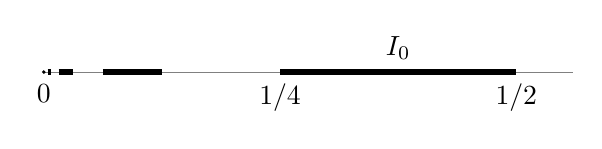
\begin{tikzpicture}[x=12cm,y=1cm]
\draw[gray] (0,0)--(.56,0);
\draw[line width=2pt] (.25,0)--(.5,0);
\draw[line width=2pt] (.0625,0)--(.125,0);
\draw[line width=2pt] (.015625,0)--(.03125,0);
\draw[line width=2pt] (.00390625,0)--(.0078125,0);
\fill (0,0) circle[radius=.7pt];
\node[below] at (0,-.03) {\(0\)};
\node[below] at (.25,-.03) {\(1/4\)};
\node[below] at (.5,-.03) {\(1/2\)};
\node[above] at (.375,.03) {\(I_0\)};
\end{tikzpicture}
\caption{Four of the infinitely many intervals in \(\Gamma\).
The intervals and gaps repeat by a factor \(q=1/4\) toward zero.}
\label{fig:screen}
\end{figure}

\section{A repeating harmonic function}\label{sec:mode}

Put \(L=\log4\) and
\[
 Q=(\R/L\mathbb Z)\times(0,\pi),\qquad
 D=\{(s,0):L/2<s<L\}.
\]
Let \(V\subset H^1(Q;\R)\) consist of functions with zero trace on \(D\).
The coordinate \(s\) is periodic. All remaining bottom boundary points and
the top boundary have the natural Neumann condition. For \(0\le a\le1/2\),
define
\begin{equation}\label{eq:form}
 b_a(u,v)=\int_Q\nabla u\cdot\nabla v+2a\int_Q u_s v .
\end{equation}
The corresponding differential operator is
\(L_a=-\Delta+2a\partial_s\). The parameter \(a\) will become a radial
exponent.

\begin{lemma}\label{lem:principal}
For every \(a\in[0,1/2]\), the weak inverse \(K_a=L_a^{-1}\) on \(L^2(Q)\)
is compact, positive and ideal-irreducible. There are
\(\lambda(a)>0\) and nonnegative nonzero \(h_a,v_a\in V\) such that
\begin{align}
 b_a(h_a,w)&=\lambda(a)\int_Qh_aw,\label{eq:eigen-direct}\\
 b_a(w,v_a)&=\lambda(a)\int_Qwv_a,\qquad w\in V.\label{eq:eigen-adjoint}
\end{align}
Both functions are strictly positive in the interior and on the open
Neumann portions of the boundary.
\end{lemma}
\begin{proof}
The bottom trace is bounded in \(H^1\), as follows by integrating
\(u(s,0)=u(s,\theta)-\int_0^\theta u_\theta(s,\tau)\dd\tau\).
The embedding \(H^1(Q)\subset L^2(Q)\) is compact: Fourier series in \(s\)
and cosine series in \(\theta\) give a uniformly small \(L^2\) tail after
finite frequency truncation. Hence
\[
 \|u\|_2\le C_P\|\nabla u\|_2,\qquad u\in V.
\]
Otherwise a normalized sequence with gradients tending to zero would
converge in \(H^1\) to a nonzero constant with zero trace on \(D\).

Periodicity gives \(\int_Q u_su=0\). With the gradient inner product on
\(V\), Riesz representation \cite[Theorems 180 and 184]{MIT} represents
the drift form by a bounded skew-adjoint operator \(T_a\).
Thus \eqref{eq:form} corresponds to \(I+T_a\). The estimate
\(\|(I\pm T_a)u\|_V\ge\|u\|_V\) gives a closed range and a zero adjoint
kernel, so \(I+T_a\) is invertible. Consequently, for each \(f\in L^2(Q)\)
there is a unique \(u=K_af\in V\) with
\(b_a(u,w)=\int_Qfw\). Its \(H^1\) bound and the compact embedding prove
compactness on \(L^2\).

If \(f\ge0\), testing by \(u^-=\max(-u,0)\in V\) gives
\[
 -\|\nabla u^-\|_2^2=\int_Q f u^-\ge0,
\]
because the drift term is zero. Thus \(u\ge0\).
For \(f\ne0\), strict interior positivity can be verified locally.
The gauge \(w=e^{-as}u\) satisfies
\((-\Delta+a^2)w=e^{-as}f\ge0\).
Cutoff and Fourier inversion give \(H^2_{\rm loc}\) regularity, hence
continuity. If \(a>0\), the function \(w(s,\theta)\cos(ay)\) is nonnegative
on a thin three-dimensional cylinder and has nonpositive distributional
Laplacian. Its mean-value inequality follows by mollification. A zero
interior value forces it to vanish nearby and then throughout the connected
domain. The case \(a=0\) uses \(w\) directly. This would force \(f=0\),
so \(K_af>0\) in the interior.

Any nonzero invariant closed ideal contains \(f\ge0\), \(f\ne0\), and
hence \(K_af>0\) almost everywhere. For \(g\in L^2\), the functions
\(\operatorname{sign}(g)\min(|g|,mK_af)\) lie in this ideal and converge
to \(g\). Thus the ideal is all of \(L^2\).
The compact irreducible Banach-lattice theorem
\cite[Theorem 1.5]{CWW} applies: the spectral radius of \(K_a\) is positive
and has positive direct and strictly positive adjoint eigenvectors.
Taking its reciprocal gives \(\lambda(a)\).
The weak inverse and its adjoint map \(L^2\) into \(V\), giving
\eqref{eq:eigen-direct}--\eqref{eq:eigen-adjoint}.
Interior bootstrapping gives smoothness. On an open Neumann portion, even
reflection preserves the constant-coefficient equation because the drift
is tangential. The same minimum argument gives positivity there.
\end{proof}

\begin{lemma}\label{lem:exponent}
The function \(\lambda(a)\) is continuous on \([0,1/2]\), and there is
\(\alpha\in(0,1/2)\) with \(\lambda(\alpha)=\alpha^2\).
\end{lemma}
\begin{proof}
The smooth function \(\phi(s,\theta)=\sin(\theta/2)\) belongs to \(V\).
It has no \(s\)-derivative, satisfies \(-\phi_{\theta\theta}=\phi/4\),
and has outward normal derivative zero at the top and \(-1/2\) at the
bottom. The adjoint equation therefore gives
\begin{equation}\label{eq:boundary-deficit}
 \lambda(a)\int_Q\phi v_a
 =\frac14\int_Q\phi v_a-\frac12\int_0^{L/2}v_a(s,0)\dd s .
\end{equation}
The last integral is strictly positive. Thus \(\lambda(a)<1/4\).
Testing the direct equation with \(h_a\) also gives
\[
 \lambda(a)\|h_a\|_2^2=\|\nabla h_a\|_2^2,
 \qquad \lambda(a)\ge C_P^{-2}>0 .
\]

If \(a_m\to a\), normalize \(\|h_{a_m}\|_2=1\).
Along a subsequence the uniform \(H^1\) bound gives weak \(H^1\) and strong
\(L^2\) convergence to \(h\ge0\), \(\|h\|_2=1\), and
\(\lambda(a_m)\to\ell\). Passing to the form equation yields
\(b_a(h,w)=\ell\int_Qhw\). Pairing with \(v_a\) shows
\[
 (\ell-\lambda(a))\int_Qhv_a=0 .
\]
The integral is positive, so every convergent subsequence has
\(\ell=\lambda(a)\). This proves continuity.
At zero, \(\lambda(0)>0\), whereas
\(\lambda(1/2)-(1/2)^2<0\). The intermediate value theorem supplies
the required root.
\end{proof}

Fix such an \(\alpha\), write \(h=h_\alpha\), and extend \(h\) periodically
in \(s\). For \(r>0\), \(0\le\theta\le\pi\), set
\begin{equation}\label{eq:mode}
 U(r,\theta)=r^\alpha h(-\log r,\theta).
\end{equation}
Extend \(U\) evenly across the real axis. Let
\[
 E=\bigcup_{j\in\mathbb Z}[q^{j+1},2q^{j+1}]
\]
on the positive real axis. The Dirichlet part of the cylinder corresponds
to these intervals, while the Neumann part corresponds to the gaps.

\begin{lemma}\label{lem:harmonic}
The function \(U\) is positive and harmonic on \(\R^2\setminus(E\cup\{0\})\),
has zero screen trace, and satisfies
\begin{equation}\label{eq:scaling}
 U(qz)=q^\alpha U(z).
\end{equation}
It extends to an \(H^1_{\rm loc}\) function at zero. Moreover, away from
zero it satisfies the weak Dirichlet energy identity for all compactly
supported \(H^1\) tests with zero screen trace.
\end{lemma}
\begin{proof}
For \(u(s,\theta)=e^{-\alpha s}h(s,\theta)\),
\[
 (\partial_s^2+\partial_\theta^2)u
     =e^{-\alpha s}(-L_\alpha h+\alpha^2h)=0 .
\]
Neumann reflection through the gaps and the negative axis gives the
claimed harmonic function. To retain the weak equation at mixed junctions,
let \(v\) be a compactly supported \(H^1\) test on the unrolled half-strip,
with zero trace on the repeated Dirichlet intervals. Periodize
\(w=e^{-\alpha s}v\) by its finite sum of translates by \(L\), and test the
eigenvalue equation. Expanding \(w_s\) gives
\[
 0=\int e^{-\alpha s}
   (h_s v_s+h_\theta v_\theta+\alpha h_s v-\alpha^2h v).
\]
Compact support in \(s\) permits integration by parts:
\[
 \int-\alpha e^{-\alpha s}h v_s
       =\int e^{-\alpha s}(\alpha h_s-\alpha^2h)v .
\]
The result is \(\int(u_sv_s+u_\theta v_\theta)=0\).
The conformal polar change converts this to planar Dirichlet energy;
even reflection combines the upper and lower tests. This proves the weak
assertion without imposing smoothness at the junctions.

Periodicity gives \eqref{eq:scaling}. The energy in
\(q^{j+1}<|z|<q^j\) is \(q^{2j\alpha}\) times that in \(q<|z|<1\);
the \(L^2\) norm squared is multiplied by \(q^{j(2\alpha+2)}\).
Both series converge. Removing a disk of radius \(q^j\) by a rescaled
fixed smooth cutoff changes the \(H^1\) norm by \(O(q^{j\alpha})\),
including the cutoff-gradient term. These truncated functions prove the
\(H^1_{\rm loc}\) extension across zero.
\end{proof}

\begin{remark}
With an entirely Dirichlet bottom boundary, the boundary term in
\eqref{eq:boundary-deficit} disappears. The familiar function
\(r^{1/2}\sin(\theta/2)\) has exponent \(1/2\).
The open gaps are what make the strict smaller exponent possible.
\end{remark}

\section{The charge and its Sobolev regularity}\label{sec:charge}

The distributional Laplacian of \(U\) will give the charge. Its positivity,
finite mass and behavior at zero must be established before using it in a
single-layer integral.

For a nonnegative smooth compactly supported test \(\zeta\) and
\(\delta>0\), use the bounded Dirichlet test
\(\zeta U/(U+\delta)\) in Lemma~\ref{lem:harmonic}. A logarithmic radial
cutoff first removes zero; its gradient has \(L^2\) norm tending to zero,
so the extra term vanishes by Cauchy--Schwarz and the finite energy of
\(U\). Thus
\[
 0=\int\nabla U\cdot\nabla\zeta\,\frac{U}{U+\delta}
    +\int\zeta\,\frac{\delta|\nabla U|^2}{(U+\delta)^2}.
\]
The second term is nonnegative. Letting \(\delta\downarrow0\) in the first
term gives \(\int\nabla U\cdot\nabla\zeta\le0\).
Consequently \(\Delta U\) is a positive distribution, supported on
\(E\cup\{0\}\).

Choose a nonnegative smooth radial cutoff \(\chi\), equal to one for
\(r\le3/5\) and zero for \(r\ge9/10\). Its derivatives lie strictly in
the screen-free annulus \(1/2<r<1\), where \(U\) is smooth. Set
\begin{equation}\label{eq:compact-charge}
 W=\chi U,\qquad \mu=\chi\Delta U,\qquad
 F=2\nabla\chi\cdot\nabla U+(\Delta\chi)U .
\end{equation}
Then
\begin{equation}\label{eq:laplacian}
 W\in H^1_c(\R^2),\quad F\in C^\infty_c(\R^2),\quad
 \Delta W=\mu+F,\quad \supp\mu\subset\Gamma\times\{0\}.
\end{equation}

\begin{lemma}\label{lem:measure}
The distribution \(\mu\) is a finite positive measure
\(\nu\otimes\delta_0\), with \(\nu\) supported on \(\Gamma\).
The measure \(\nu\) is nonzero on every open subinterval of \(I_0\), and
\begin{equation}\label{eq:charge-scaling}
 \nu(q^j A)=q^{j\alpha}\nu(A),\qquad A\subset I_0,\quad j\ge0 .
\end{equation}
\end{lemma}
\begin{proof}
Positivity gives an order-zero bound on every fixed compact set:
if \(\beta\ge0\) is smooth and at least one on the support of a real
test \(f\), then
\[
 |\langle\mu,f\rangle|\le\langle\mu,\beta\rangle\|f\|_\infty .
\]
Choose \(\omega\ge0\) smooth and compactly supported in the normal
coordinate, equal to one near zero, and define the positive distribution
\(\langle\nu,\psi\rangle=\langle\mu,\psi(x)\omega(y)\rangle\) on \(\R\).
The positive-distribution representation theorem
\cite[Proposition 1.9.11 and Remark 1.9.12]{Nonn} makes \(\nu\) a locally
finite positive measure. Its compact support makes it finite.

For a planar test \(f\), the function
\(g(x,y)=f(x,y)-f(x,0)\omega(y)\) vanishes on the line.
Multiplying it by a cutoff supported in \(|y|\le h\), equal to one near
zero, does not change its pairing with \(\mu\).
The sup norm of this product tends to zero as \(h\downarrow0\).
The order-zero bound therefore gives \(\langle\mu,g\rangle=0\),
proving \(\mu=\nu\otimes\delta_0\).

If the measure vanished on an open subinterval of \(I_0\), then
\(\Delta U=0\) in a full neighborhood of that subinterval.
The nonnegative function \(U\) would be harmonic there and have zero
trace on the line. The interior minimum principle would force it to
vanish, contrary to positivity above the screen. Finally,
\eqref{eq:scaling} implies that the distributional charge on a scaled
planar set is multiplied by \(q^\alpha\): the area Jacobian cancels the
two derivatives. Since \(\chi=1\) on all \(I_j\), this gives
\eqref{eq:charge-scaling}.
\end{proof}

\begin{lemma}\label{lem:regularity}
The measure \(\nu\) belongs to \(H^{-1/2}_\Gamma(\R)\), has no atom at
zero, and fails to belong to \(H^{-\varepsilon}(\R)\) for every
\(0<\varepsilon<1/2-\alpha\).
\end{lemma}
\begin{proof}
Equation~\eqref{eq:laplacian} gives \(\mu\in H^{-1}(\R^2)\).
The unitary Fourier convention yields
\(\widehat\mu(\xi,\eta)=(2\pi)^{-1/2}\widehat\nu(\xi)\).
Since
\(\int_\R(1+\xi^2+\eta^2)^{-1}\dd\eta=\pi(1+\xi^2)^{-1/2}\),
\begin{equation}\label{eq:energy-line}
 \|\mu\|_{H^{-1}(\R^2)}^2
       =\tfrac12\|\nu\|_{H^{-1/2}(\R)}^2 .
\end{equation}
This proves energy membership.
A smooth logarithmic cutoff \(\eta_r\), equal to one for \(|z|\le r^2\)
and zero for \(|z|\ge r\), has
\(\|\eta_r\|_{H^1}\to0\): radial integration bounds its squared gradient
norm by \(C/|\log r|\).
Positivity and \(H^{-1}\) duality give
\(\mu(\{0\})\le\|\mu\|_{H^{-1}}\|\eta_r\|_{H^1}\to0\).
Thus compactification has introduced no origin delta.

Choose a nonnegative \(\psi\in C^\infty_c(\operatorname{int}I_0)\) with
\(M=\int\psi\dd\nu>0\), and put \(\psi_j(x)=\psi(q^{-j}x)\).
Then
\[
 \langle\nu,\psi_j\rangle=q^{j\alpha}M,\qquad
 \|\psi_j\|_{H^\varepsilon}
       \le q^{j(1/2-\varepsilon)}\|\psi\|_{H^\varepsilon}.
\]
Indeed \(\widehat\psi_j(\xi)=q^j\widehat\psi(q^j\xi)\), and changing
variables in the Fourier norm gives the latter inequality.
If \(\nu\in H^{-\varepsilon}\), duality would bound the first quantity
by a fixed multiple of the second. Their ratio tends to infinity because
\(\alpha-1/2+\varepsilon<0\).
\end{proof}

By \eqref{eq:trace-adjoint}, there is a unique
\begin{equation}\label{eq:density}
 \Psi\in\hH^{-1/2}(\Gamma),\qquad \tr_\Gamma^*\Psi=\nu .
\end{equation}
Compatibility of the adjoint trace maps shows from
Lemma~\ref{lem:regularity} that
\begin{equation}\label{eq:density-failure}
 \Psi\notin\hH^{-\varepsilon}(\Gamma)
 \quad(0<\varepsilon<1/2-\alpha).
\end{equation}
This uses the original quotient duals, not a new density space.

\section{The Helmholtz image and failure of surjectivity}\label{sec:image}

Let \(G(z)=-(2\pi)^{-1}\log|z|\), so that \(\Delta G=-\delta_0\).
Convolving \eqref{eq:laplacian} gives
\begin{equation}\label{eq:potential}
 G*\mu=-W-G*F .
\end{equation}
The equality is distributional: \(W\) is compactly supported and
\(G*\Delta W=(\Delta G)*W=-W\). The volume potential \(G*F\) is smooth.
Since the line trace of \(W\) vanishes on \(\Gamma\), the Laplace
single-layer image is the restriction of the smooth line function
\[
 P_0(x)=-(G*F)(x,0).
\]

For clarity, this trace identity is continuous at the exact energy
regularity. Localize \(G\) by a smooth cutoff equal to one on all
differences of a fixed neighborhood of the screen and the screen.
For the compact kernel \(K\),
\((1-\Delta)K=\delta_0+R\), \(R\in L^1(\R^2)\).
Hence its Fourier multiplier is \(O((1+|\xi|^2)^{-1})\), and convolution
maps \(H^{-1}\) to \(H^1\). Fourier inversion in the normal variable,
followed by Cauchy--Schwarz, gives the trace bound
\(H^1(\R^2)\to H^{1/2}(\R)\). Thus \eqref{eq:potential} holds in the
required trace space.

The change to positive \(k\) does not destroy the smooth-enough data.
On the supporting line put
\[
 D_k(x)=\Phi_k((x,0))+\frac1{2\pi}\log|x|.
\]
The exact Bessel formulas \cite[10.2.2, 10.4.3, 10.8.2]{DLMF} give,
near zero,
\begin{equation}\label{eq:bessel}
 D_k(x)=\kappa_k+A_k(x^2)+x^2\log|x|B_k(x^2),
\end{equation}
where \(\kappa_k\in\mathbb C\), \(A_k,B_k\) are analytic and \(k>0\) is fixed.
In particular \(D'_k(x)=O(|x|(1+|\log|x||))\to0\); the even extension
is \(C^1\) at zero.
Multiply by a smooth cutoff equal to one for \(|x|\le1\), obtaining
\(d_k\in C^1_c(\R)\). Because \(\nu\) is a finite measure,
dominated differentiation and uniform continuity of \(d'_k\) give
\begin{equation}\label{eq:correction}
 (d_k*\nu)'=d'_k*\nu,\qquad
 d_k*\nu\in C^1_c(\R)\subset H^1(\R).
\end{equation}

We also need continuity for the density approximation identifying the
original operator. Since \(d_k,d'_k\in L^1\), integration by parts gives
\[
 |\widehat d_k(\xi)|\le C_k(1+\xi^2)^{-1/2}.
\]
Thus convolution with \(d_k\) is continuous
\(H^{-1/2}\to H^{1/2}\). Bounded densities are dense in the energy space
by \cite[Theorem 2.7]{CGH}. For each such density, the integral
representation \cite[Theorem 4.6]{CGH} is the sum of its localized
Laplace line potential and its \(d_k\) correction.
The localized planar potentials converge in \(H^1\), their line traces
in \(H^{1/2}\), and the corrections in \(H^{1/2}\).
Passing to the original continuous extension therefore proves
\begin{equation}\label{eq:original-image}
 \mathbb S_k\Psi=\tr_\Gamma(P_0+d_k*\nu).
\end{equation}
After multiplying \(P_0\) by a smooth cutoff equal to one near \(\Gamma\),
the right-hand side has an \(H^1(\R)\) extension by
\eqref{eq:correction}.

\begin{proof}[Proof of Theorem~\ref{thm:main}]
Lemma~\ref{lem:ahlfors} gives the admissible compact \(1\)-set.
Fix \(\alpha\) from Lemma~\ref{lem:exponent} and \(\Psi\) from
\eqref{eq:density}; both are independent of \(k\).
For \(\alpha<t<1/2\), put \(\varepsilon=1/2-t\).
Then \(0<\varepsilon<1/2-\alpha\), and
\(g_k=\mathbb S_k\Psi\) belongs to
\(\hH^{1-\varepsilon}(\Gamma)=\hH^{t+1/2}(\Gamma)\).
If \(Z\in\hH^{-\varepsilon}(\Gamma)\) had \(\mathbb S_k Z=g_k\),
the continuous embedding
\(\hH^{-\varepsilon}(\Gamma)\subset\hH^{-1/2}(\Gamma)\) and
\eqref{eq:coercive} would give \(Z=\Psi\).
This contradicts \eqref{eq:density-failure}.
\end{proof}

\begin{thebibliography}{9}
\bibitem{CGH}
A. M. Caetano, S. N. Chandler-Wilde, A. Gibbs, D. P. Hewett and A. Moiola,
\emph{A Hausdorff-measure boundary element method for acoustic scattering
by fractal screens}, Numerische Mathematik \textbf{156} (2024), 463--532.
\href{https://doi.org/10.1007/s00211-024-01399-7}{doi:10.1007/s00211-024-01399-7}.
Preprint version used: \href{https://arxiv.org/abs/2212.06594v2}{arXiv:2212.06594v2}.

\bibitem{MF}
S. N. Chandler-Wilde, G. Claret, D. P. Hewett, A. Rozanova-Pierrat and
S. Sadeghi, \emph{Integral Equation Methods for Scattering by Multifractal
Obstacles} (2026), \href{https://arxiv.org/abs/2605.19540v1}{arXiv:2605.19540v1}.

\bibitem{CWW}
K.-C. Chang, X. Wang and X. Wu,
\emph{On the spectral theory of positive operators and PDE applications},
Discrete and Continuous Dynamical Systems \textbf{40}(6) (2020), 3171--3200.
\href{https://doi.org/10.3934/dcds.2020054}{doi:10.3934/dcds.2020054}.

\bibitem{MIT}
C. Rodriguez (lecturer), A. Lin (notes),
\emph{18.102: Introduction to Functional Analysis}, MIT OpenCourseWare,
Spring 2021, Theorems 180 and 184, pp. 90--93.
\url{https://ocw.mit.edu/courses/18-102-introduction-to-functional-analysis-spring-2021/8fb8d5c170f1613151aca71de21027bc_MIT18_102s21_full_lec.pdf}.

\bibitem{Nonn}
S. Nonnenmacher,
\emph{Lecture Notes for the course Distributions and Partial Differential
Equations}, Universit\'e Paris-Saclay, September 2022,
Proposition 1.9.11 and Remark 1.9.12, pp. 60--61.
\url{https://www.imo.universite-paris-saclay.fr/~stephane.nonnenmacher/enseign/Distributions2022_Chap1-3.pdf}.

\bibitem{DLMF}
\emph{NIST Digital Library of Mathematical Functions}, version 1.2.8,
released September 15, 2026, equations 10.2.2, 10.4.3 and 10.8.2.
\url{https://dlmf.nist.gov/}.
\end{thebibliography}

\section*{AI use}
An AI assistant, OpenAI Codex, assisted with the construction, drafting,
source checks and mathematical review. No proof-critical numerical
computation is used. Independent mathematical review is requested.

\end{document}
